\chapter{Ferramentas}
\label{ferramentas}
Nesta seção são apresentadas as tecnologias/ferramentas utilizadas no desenvolvimento do projeto. São descritas também, de forma breve, suas características, qualidades e vantagens, mostrando o porquê foram escolhidas no desenvolvimento do sistema. Foram utilizadas tecnologias robustas e já consolidadas no mercado. 
\section{Unity 2021.2.5f}
O Unity é um motor gráfico multiplataforma que é amplamente utilizado em desenvolvimento de jogos e aplicativos interativos. Ele permite que os desenvolvedores criem conteúdo 3D e 2D de alta qualidade com uma ampla variedade de ferramentas e recursos, incluindo renderização de última geração, física realista, animação, iluminação e efeitos de partículas. Além disso, o Unity possui uma comunidade ativa e uma ampla variedade de recursos de aprendizado, o que o torna uma opção atraente para desenvolvedores iniciantes e experientes.

O Unity também é conhecido por sua ampla compatibilidade com dispositivos e plataformas, incluindo PC, Mac, dispositivos móveis, consoles de videogame e realidade virtual. Isso permite que os desenvolvedores criem conteúdo para uma ampla gama de públicos e dispositivos, aumentando assim o alcance de seus projetos. Além disso, o Unity possui integração com ferramentas de terceiros, como o GitHub, o que facilita o trabalho em equipe e o gerenciamento de projetos de desenvolvimento. \cite{unity}
\pagebreak
\subsection{Tile Palette e TileMaps}
Ferramenta auxiliadora para o desenho de Tiles pelo cenário. Tiles são unidades de imagem que representam algo. Exemplo: 
\begin{figure}[!h]
    \centering
    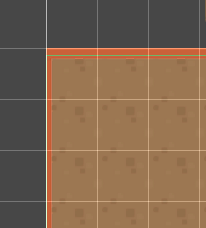
\includegraphics[width=200px]{figuras/tiles.png}
    \caption{Tiles}
    \label{fig_tiles}
\end{figure}
Cada pequeno quadrado é um Tile, e junção de tais Tiles formam algo, como uma plataforma, o chão, um obstáculo. E esta ferramenta auxilia podendo desenhar tais formatos que estes tiles serão arranjados pelo cenário. 
\footnote{Mais informações: \url{https://www.youtube.com/watch?v=ryISV_nH8qw&ab_channel=Brackeys}} 
\footnote{Mais informações: \url{https://github.com/Unity-Technologies/2d-extras}}
\footnote{Mais informações: \url{https://docs.unity3d.com/Manual/Tilemap-Palette.html}}

\subsection{Localization}
Ferramenta auxiliadora para a adição de idiomas no jogo. Por meio de tabelas que representam entidades. Como por exemplo a tabela de itens. \footnote{Mais informações: \url{https://docs.unity3d.com/Packages/com.unity.localization@1.0/manual/index.html}}
\begin{table}[h]
    \centering
    \begin{tabular}{|l|l|l|}
        \hline
          & português        & inglês      \\ \hline
        0 & ferro            & iron        \\ \hline
        1 & ouro             & gold        \\ \hline
    \end{tabular}
\caption{Tabela de exemplo Localzation}
\label{table:localization}
\end{table}
Neste exemplo, durante o desenvolvimento do jogo, em situações onde textos devem ser traduzidos, podemos referenciar os nomes pelo ID da tabela, e o jogo a partir do momento em que está localizado em algum idioma, substitui a referência do texto pela sua versão do idioma selecionado.

\subsection{Animator}
Ferramenta nativas do Unity para inserção de animações nos jogos, por meio desta ferramenta podemos encadear ações para iniciar uma animação específica, como por exemplo: Ao apertar o botão Espaço devemos sair da animação padrão para a animação de pulo. A partir de uma máquina de estados de animações.\footnote{Mais informações: \url{https://docs.unity3d.com/ScriptReference/Animator.htmll}}
\begin{figure}[!h]
    \centering
    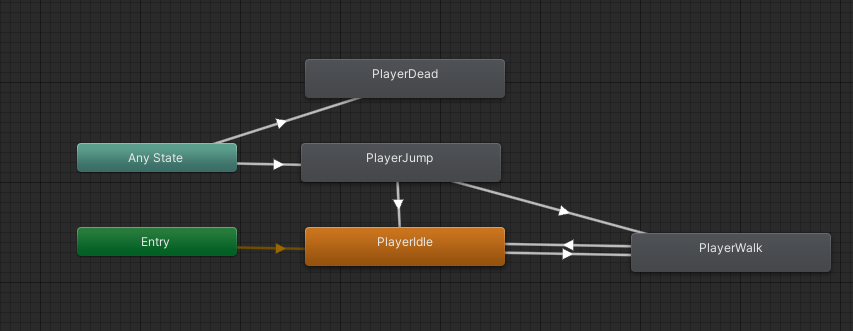
\includegraphics[width=400px]{figuras/animator.png}
    \caption{Exemplo de animator do personagem Weee}
    \label{fig_animator}
\end{figure}
Neste exemplo, a animação padrão é PlayerIdle, e a partir desta animação podemos ir para PlayerWalk. Em PlayerWalk podemos voltar para PlayerIdle ou ir para PlayerJump. Em PlayerJump podemos voltar para PlayerIdle. A partir de qualquer estado podemos ir para PlayerJump ou PlayerDead

\section{Linguagens de Programação}
C\# é uma linguagem de programação orientada a objetos desenvolvida pela Microsoft. Ela é amplamente utilizada em aplicativos de desktop, aplicativos móveis, jogos e sistemas web. C\# possui uma sintaxe semelhante a outras linguagens de programação como C++ e Java, o que a torna fácil de aprender para aqueles já familiarizados com essas linguagens. Além disso, C\# possui uma ampla variedade de recursos e bibliotecas, como suporte ao .NET Framework, que tornam mais fácil para os desenvolvedores criarem aplicativos de alta qualidade e funcionalidade.
\par
C\# é uma linguagem de programação de alto nível, o que significa que ela é mais fácil de ler e escrever do que linguagens de baixo nível como o Assembly. Isso a torna uma opção atraente para aqueles que desejam criar aplicativos complexos sem se preocupar tanto com os detalhes de baixo nível.
\par
C\# também possui um forte suporte à programação paralela, o que permite que os desenvolvedores criem aplicativos que aproveitam ao máximo a potência dos processadores multicore. Além disso, C\# é uma linguagem de programação compilada, o que significa que o código é convertido em um formato de máquina antes de ser executado. Isso pode levar a um desempenho ligeiramente superior em comparação com linguagens interpretadas, como Python.

\section{Formato de Jogo}
O jogo será no formato 2D com mini games que serão jogos digitalizados baseados nos jogos físicos presentes em \cite{bell1998computerIHC}
Neste trabalho, pretende-se auxiliar na absorção do conteúdo da disciplina de forma lúdica. 